%%%%%%%%%%%%%%%%%%%%%%%%%%%%%%%%%%%%%%%%%%%%%%%%%%%%%%%%%%%%%%%%%%%%%%%%%%%%%%%
%
% Main Document
% Copyright (c) 2010 by tilo.mueller@rwth-aachen.de
% 
%%%%%%%%%%%%%%%%%%%%%%%%%%%%%%%%%%%%%%%%%%%%%%%%%%%%%%%%%%%%%%%%%%%%%%%%%%%%%%%

%%%%%%%%%%%%%%%%%%%%%%%%%%%%%%%%%%%%%%%%%%%%%%%%%%%%%%%%%%%%%%%%%%%%%%%%%%%%%%%
%
% Header
% Copyright (c) 2010 by tilo.mueller@rwth-aachen.de
% 
%%%%%%%%%%%%%%%%%%%%%%%%%%%%%%%%%%%%%%%%%%%%%%%%%%%%%%%%%%%%%%%%%%%%%%%%%%%%%%%

% Document
	% Font size and paper
	\documentclass[11pt,twoside,a4paper,fleqn]{scrbook}
	% Margin
	\usepackage{anysize}
	\marginsize{3cm}{3cm}{2cm}{2cm}
	% Font
	\usepackage[T1]{fontenc}

% Fancy header and footer
	\usepackage{fancyhdr}
	\pagestyle{fancy}
	\fancyhf{}
	% Centrical header  
	\fancyhead[C]{\textsc{\nouppercase{\leftmark}}}
	\renewcommand{\headrulewidth}{0.5pt}
	% Centrical footer
	\fancyfoot[C]{\thepage}
	\renewcommand{\footrulewidth}{0pt}

% Fancy chapter page
	% fncychap: Sonny Lenny Glenn Conny Rejne Bjarne Bjornstrup PetersLenny
	%\usepackage[PetersLenny]{fncychap}
	% or titlesec:
	%\usepackage{titlesec}
	%\titleformat{\chapter}{\bf\Huge}{\thechapter\quad}{0em}{}
	% or:
	\makeatletter
	\def\@makechapterhead#1{
	  \vspace*{100\p@}
	  {\parindent \z@ 
	    {\raggedleft %\reset@font
	      \fontsize{15ex}{15ex}%\selectfont
	      \textsf\thechapter\par\nobreak}
	    \par\nobreak
	    \interlinepenalty\@M
	    {\raggedright \Huge \textsf{\textsc{#1}}}
	    \par\nobreak
	    \leavevmode \leaders \hrule height 0.65ex \hfill \kern \z@
	    \par\nobreak
	    \vskip 100\p@
	  }
	}

% Fancy toc title
	% \renewcommand{\contentsname}{CONTENTS}
	% or:
	\def\tableofcontents{
		\section*{
			\centering Inhalt
		}
		\@starttoc{toc}
	}

% Language, character set
	% Umlauts
	% \usepackage[latin1]{inputenc}
	\usepackage[utf8]{inputenc}
	% Phonetics
	% \usepackage[safe]{tipa}
	% Symbols
	% \usepackage{latexsym}

% Figures
	% Graphics
	\usepackage[]{graphicx,float,subfigure} 
	% Frame 
	\usepackage{fancybox}
	% Code listings
	\usepackage{listings,algorithm,algorithmic}
	% Image subdir
	\graphicspath{{images/}}
	% Formatting captions
	\usepackage[small,indent]{caption}

% Bibliography
%\usepackage[sectionbib]{natbib}
%\usepackage{chapterbib}
\usepackage{cite}

% Links within pdf file
	\usepackage[]{hyperref}
	\hypersetup{
		colorlinks=true,
		linkcolor=blue,
		citecolor=blue,
		filecolor=blue,
		pagecolor=blue,
		urlcolor=blue,
		breaklinks=true,
		bookmarksnumbered=true,
		pdfstartpage={1},
		pdftitle={TITLE}, %TODO
		pdfsubject={SUBJECT}, %TODO
		pdfauthor={AUTHOR}, %TODO
		pdfproducer={LaTex with hyperref}
	}

% Misc
	% Appendix
	\usepackage{appendix}
	% Date
	\usepackage{times}
	% Glossary
	\usepackage[refpage]{nomencl}
	%Index 
	\usepackage{makeidx}
	\makeindex
	% Math
	\usepackage{amssymb,amsfonts,amsmath}
	% Allow the use of underscore in normal text
	\usepackage{underscore}
	% Hyphenation
	\hyphenation{donothyphenatethisword}
	% Longtables
	\usepackage{longtable}
	% multicolumn
	\usepackage{multirow}

% Commands
	% new introduced terms
	\newcommand{\new}[1]{\textit{#1}}
	% code terms
	\newcommand{\code}[1]{\texttt{#1}}
	% comment out multiple lines
	\newcommand{\ignore}[1]{}


% No headers on empty pages before new chapter
\makeatletter
\def\cleardoublepage{\clearpage\if@twoside \ifodd\c@page\else
    \hbox{}
    \thispagestyle{plain}
    \newpage
    \if@twocolumn\hbox{}\newpage\fi\fi\fi}
\makeatother \clearpage{\pagestyle{plain}\cleardoublepage}


\begin{document}

% a)
	% Alphabetic page numbers
	\pagenumbering{alph}

	% Title 
	%%%%%%%%%%%%%%%%%%%%%%%%%%%%%%%%%%%%%%%%%%%%%%%%%%%%%%%%%%%%%%%%%%%%%%%%%%%%%%%
%
% Title
% Copyright (c) 2010 by tilo.mueller@rwth-aachen.de
% 
%%%%%%%%%%%%%%%%%%%%%%%%%%%%%%%%%%%%%%%%%%%%%%%%%%%%%%%%%%%%%%%%%%%%%%%%%%%%%%%

\begin{titlepage}

\titlehead{
	\center{
		\begin{tabular}[ht]{lcr}
			\parbox{3cm}{\center{
				
\includegraphics[height=1cm]{fau.png}
			}}
			&
			\parbox{5cm}{\center{
				Lehrstuhl für Informatik 1
				Friedrich-Alexander-Universität\\ 
				Erlangen-Nürnberg
			}}
			&
			\parbox{3cm}{\center{
				
\includegraphics[height=1cm]{i1.png}
			}}
		\end{tabular}
		\vspace{4em}
	}
}

\subject{
	BACHELOR THESIS
}

\title{
	Der Kompromiss zwischen Privatsphäre und Dienstleistungen am Beispiel Google\\
}

\author{
	\vspace{4em}
	\\
	Richard Baumann\\
} 

\date{
	Erlangen, 
	\today
} 

\publishers{\center{\parbox{0cm}{
	\begin{tabbing}
		xxxxxxxxxxxxxxxxxxxxx\=xxxxxxxxxxxxxxxxxxxxxxxxx\kill
		First Examiner:	\> Prof. Dr. Felix Freiling\\
		Advisor:		\> Nadina Hintz\\
		Advisor:        \> Zinaida Benenson
	\end{tabbing}
}}}

\maketitle
\end{titlepage}



%%%%%%%%%%%%%%%%%%%%%%%%%%%%%%%%%%%%%%%%%%%%%%%%%%%%%%%%%%%%%%%%%%%%%%%%%%%%%%%
% Example for handwritten title page
% (might be more flexible)
\ignore{
\begin{titlepage}
\center
% Title
\vspace{4em}
\Large{{BACHELOR THESIS}}\\
\vspace{2em}
\Huge{\textsf{THEMA}}\\
% Name
\vspace{2em}
\LARGE{
	Tilo Müller\\
	\today\\
}
% Examiners, Advisors
\vspace{8em}
\large{
	\textsf{
		Second Examiner:	Prof. Dr. Felix Freiling\\
		Advisor:		Tilo Müller\\
	}
}
\end{titlepage}
\pagestyle{empty} \mbox{} \clearpage
}


% i)
	% Roman page numbers; alternative: \pagenumbering{off}
	\pagenumbering{roman}

	% No indent for paragraphs
	\setlength{\parskip}{1.3ex plus 0.2ex minus 0.2ex}
	\setlength{\parindent}{0pt}

	% Pre content
	%%%%%%%%%%%%%%%%%%%%%%%%%%%%%%%%%%%%%%%%%%%%%%%%%%%%%%%%%%%%%%%%%%%%%%%%%%%%%%%
%
% Declaration 
% Copyright (c) 2010 by tilo.mueller@rwth-aachen.de
% 
%%%%%%%%%%%%%%%%%%%%%%%%%%%%%%%%%%%%%%%%%%%%%%%%%%%%%%%%%%%%%%%%%%%%%%%%%%%%%%%


% Pseudo chapter
\chapter*{\ }


% Horizontal line
\vspace*{\fill}
%\hline
%\vspace{1.5em}


% Header
\begin{Large}
	\textbf{Eidesstattliche Erklärung / Statutory Declaration}
\end{Large}
\vspace{1.5em}


% German
Hiermit versichere ich eidesstattlich, dass die vorliegende Arbeit von mir selbstständig, ohne Hilfe Dritter und ausschließlich unter Verwendung der angegebenen Quellen angefertigt wurde. Alle Stellen, die wörtlich oder sinngemäß aus den Quellen entnommen sind, habe ich als solche kenntlich gemacht. Die Arbeit wurde bisher in gleicher oder ähnlicher Form keiner anderen Prüfungsbehörde vorgelegt. 
\vspace{1.5em}


% Header
%\begin{Large}
%	\textbf{Statutory Declaration}
%\end{Large}
%\vspace{1.0em}


% English
I hereby declare formally that I have developed and written the enclosed thesis entirely by myself and have not used sources or means without declaration in the text. Any thoughts or quotations which were inferred from the sources are marked as such. This thesis was not submitted in the same or a substantially similar version to any other authority to achieve an academic grading. 
\vspace{2em}


% Sign
Erlangen, \today\\
\begin{flushright}
	\underline{\ \ \ \ \ \ \ \ \ \ \ \ \ \ \ \ \ \ \ \ \ \ \ \ \ 
		\ \ \ \ \ \ \ \ \ \ \ \ \ \ \ \ \ \ \ \ \ \ \ \ \ \ \ \ \ 
	}\\
	\small{Richard Baumann}
\end{flushright}

	%%%%%%%%%%%%%%%%%%%%%%%%%%%%%%%%%%%%%%%%%%%%%%%%%%%%%%%%%%%%%%%%%%%%%%%%%%%%%%%
%
% Abstract
% Copyright (c) 2010 by tilo.mueller@rwth-aachen.de
% 
%%%%%%%%%%%%%%%%%%%%%%%%%%%%%%%%%%%%%%%%%%%%%%%%%%%%%%%%%%%%%%%%%%%%%%%%%%%%%%%

% Pseudo chapter
\chapter*{\ }


\begin{center}
	\begin{large}
		\textbf{Zusammenfassung}
	\end{large}
\end{center}
\vspace{0.75em}
Google Dienste werden heutzutage von vielen Personen genutzt, teilweise sogar fest in das tägliche Leben integriert. 
Mit den in letzter Zeit häufiger werdenden Datenschutzbedenken und dem von Snowden veröffentlichten Material sollte man sich genaue Überlegungen zum Datenschutz machen. 

Auf der anderen Seite kann der Nutzer auch eingeschränkt werden, wenn er seine Daten nicht an Google weitergibt. So funktionieren zum Beispiel personalisierte Suchergebnisse nur, wenn die Suchmaschine auch tatsächlich Informationen über den Nutzer hat.

Diese Arbeit soll untersuchen ob es auf Seiten der Nutzer einen Konflikt zwischen dem Angebot an Diensten durch Google und der Privatsphäre gibt. Dazu wurden im Verlauf der Arbeit zwei Forschungsfragen beantwortet: \glqq Wie viel wissen Nutzer von der Datensammlung durch Google?\grqq\ und \glqq Treffen sie Maßnahmen um gegen dieses Sammeln von Daten vorzugehen?\grqq .

Um diese Fragen zu beantworten wurde ein Fragebogen mit 39 Fragen entworfen und über verschiedene Methoden verteilt. Nachdem über 800 vollständig ausgefüllte Fragebögen abgegeben wurden wurde die Umfrage beendet und mit der Auswertung begonnen. Dabei wurden Hypothesen falls möglich belegt und danach die Forschungsfragen beantwortet. 

Dabei kam heraus, dass das typische Paradoxon der Privatsphäre auch hier auftritt - die Nutzer wünschen sich zwar mehr Privatsphäre, unternehmen aber nur selten Aktionen um ihre Privatsphäre zu schützen.

Am Ende werden noch einige Ideen für zukünftige Arbeiten in diesem Themenbereich genannt, unter anderem eine Umfrage bei der auf eine homogenere Aufteilung der Bevölkerungsgruppen geachtet werden sollte.

\vspace{2em}
\begin{center}
	\begin{large}
		\textbf{Abstract}
	\end{large}
\end{center}
\vspace{0.75em}
In dieser Arbeit wurde der Konflikt zwischen Privatsphäre und der Verwendung von Google Diensten untersucht. Mithilfe einer Umfrage wurden Forschungsfragen beantwortet. Die Frage \glqq Wie viel wissen Nutzer von der Datensammlung durch Google?\grqq\ konnte damit beantwortet werden, dass bei einem Großteil der Teilnehmer Wissen vorhanden ist. Die zweite Forschungsfrage \glqq Treffen sie Maßnahmen um gegen dieses Sammeln von Daten vorzugehen?\grqq\ wurde bis auf wenige Ausnahmen negativ beantwortet. Dieser Konflikt ist mit dem \glqq Privatsphäre Paradox\grqq\ zu erklären.

	% Table of Contents
	% \setcounter{tocdepth}{1} % less details
	% \listoftables
	% \listoffigures
	% \addcontentsline{toc}{section}{References}
	\tableofcontents
	\newpage \cleardoublepage	

% 1)
	% Arabic page numbers
	\pagenumbering{arabic}

	% Fancy header / footer for chapter pages
	\fancypagestyle{plain}{
		\fancyhf{}
		\renewcommand{\headrulewidth}{0pt}
		\fancyfoot[LE,RO]{\thepage}
	}

	% Fancy header / footer for normal pages
	\pagestyle{fancy}
	\fancyhf{}
	\fancyfoot[LE,RO]{\thepage}
	\fancyhead[LO]{\leftmark}
	\fancyhead[RE]{\rightmark}

	% Actual content
	%%%%%%%%%%%%%%%%%%%%%%%%%%%%%%%%%%%%%%%%%%%%%%%%%%%%%%%%%%%%%%%%%%%%%%%%%%%%%%%
%
% Introduction
% Copyright (c) 2010 by tilo.mueller@rwth-aachen.de
% 
%%%%%%%%%%%%%%%%%%%%%%%%%%%%%%%%%%%%%%%%%%%%%%%%%%%%%%%%%%%%%%%%%%%%%%%%%%%%%%%

\chapter{Einführung}

%Section		Depth
%\part			1
%\chapter		2
%\section 		3
%\subsection 		4
%\subsubsection 	5 	-> from here on it's not in default TOC anymore
%\paragraph	 	6
%\subparagraph 		7

\section{Motivation}
Mit den vor kurzem aufgetretenen Veröffentlichungen durch Edward Snowden sind der Datenschutz und die Privatsphäre wieder zu einem relevanten Gesprächsthema geworden. So sagt zum Beispiel Hanspeter Thür, der Datenschutzbeauftragte der Schweiz: "Privatsphäre wird zu einem Privileg" \cite{nzzdatenschutzprivileg}. Durch diese Debatten geraten auch große Unternehmen im Internet wieder in den Fokus. Da auch in Deutschland die Google Inc. eine sehr große Nutzerbasis hat (alleine in Deutschland nutzen ungefähr 38 Millionen Nutzer die Suchmaschine von Google \cite{statistagoogle}), ist es logisch, dass auch sie des öfteren mit Datenschützern in Konflikt gerät (siehe zum Beispiel "Datenschützer: Google verstößt gegen geltendes Recht" \cite{gulligooglegeltendesrecht}). Die Google Suchmaschine ist dabei nicht der einzige Google Dienst der dabei in den Mittelpunkt von Diskussionen gerät. Spätestens seit Julian Assange Google eine "privatisierte NSA" genannt hat \cite{assangegooglensa}, ist es klar, dass man sich im Bezug auf persönliche Daten bei Google besonders Gedanken machen muss.\\
Dabei ist der wichtigste Aspekt der Mensch selbst - und zwar nicht die Mitarbeiter von Google oder die Datenschützer im Besonderen sondern die normalen Nutzer. Der Nutzer ist derjenige, dessen Daten von Google verwendet werden und somit derjenige der sich davor Schützen kann, oder damit leben muss dass Google die Daten besitzt.


\section{Zielsetzung und Forschungsfragen}
Diese Arbeit soll die Nutzer von Google näher betrachten und herausfinden wie diese Nutzer über ihren Datenschutz im Bezug auf Google denken und wie sie vorgehen um ihre Daten zu schützen. Hierzu wird eine Umfrage durchgeführt die Nutzer über ihr Verhalten auf Google und ihre Gedanken über Google befragt.
Die grundsätzlichen Forschungsfragen die behandelt werden sind "Wie viel wissen Nutzer von der Datensammlung durch Google?" und "Versuchen sie gegen dieses Sammeln von Daten vorzugehen?". 

\section{Kategorien zur Einordnung der Fragen}
\label{sec:categories}
Zum Aufstellen der Hypothesen und zur späteren Einteilung der Fragen des Fragebogens wurden Kategorien aufgestellt, die wie folgt definiert wurden:
\begin{enumerate}
\setcounter{enumi}{-1}
\item \label{itm:Kat0}\textbf{Nutzung von Google Diensten}: Das Nutzungsverhalten der Google Dienste von Seiten der Nutzer. Dieser Teil fragt vor allem allgemeine Daten zum Nutzungsverhalten ab. Darunter fallen unter anderem die Information, welche Dienste genutzt werden und wie viele Accounts die Nutzer haben.
\item \label{itm:Kat1}\textbf{Kenntnisse über Googles Datenschutz}: Angeeignetes Wissen über den Umgang mit personenbezogenen Daten bei Google, vor allem im Bezug auf die genutzten Dienste. Hierbei sind Fragen wie "Bietet Google auf Nutzer zugeschnittene Werbung an?" relevant.
\item \label{itm:Kat2}\textbf{Vertrauen in Google}: Das Glauben an auftrende negative Konsequenzen im Zusammenhang mit dem Preisgeben der Daten (vgl. Kim et al., 2008).
\item \label{itm:Kat3}\textbf{Wahrgenommenes Risiko für die Privatsphäre}: Das Glauben an auftretende negative Konsequenzen im Zusammenhang mit dem Preisgeben der Daten (vgl. Kim et al., 2008)
\item \label{itm:Kat4}\textbf{Aufgeben der Privatsphäre}: Das Bewusstsein über den Verlust der Privatsphäre bei der Verwendung von Google Diensten.
\item \label{itm:Kat5}\textbf{Schutzmaßnahmen}: Verhalten des Nutzers zum Schutze der eigenen Privatsphäre
\end{enumerate}

\section{Hypothesen}
Die Forschungsfragen werden beantwortet indem Hypothesen aufgestellt werden die den Zusammenhang der oben genannten Kategorien darstellen.
Die Hypothesen sind angetragen, indem zuerst die beiden Kategorien aufgelistet werden, zwischen denen die Hypothese einen Zusammenhang darstellen soll. Danach kommt eine kurze Definition der Hypothese.
Die zugehörigen zu testenden Hypothesen sind die Folgenden:
\begin{description}
\item[\label{itm:H0}\textbf{H0}] Nutzung von Google Diensten \ref{itm:Kat0} $\rightarrow$ Kenntnisse über Googles Datenschutz \ref{itm:Kat1}: Wenn eine Person Google aktiver nutzt, bekommt sie mehr Erfahrung und Kenntnisse über Google Dienste und mögliche Probleme mit der Privatsphäre
\item[\label{itm:H1}\textbf{H1}] Kenntnisse über Google \ref{itm:Kat1} $\rightarrow$ Aufgeben der Privatsphäre \ref{itm:Kat4}: Je mehr eine Person über Googles Datenschutz weiß, desto seltener gibt sie Teile ihrer Privatsphäre auf
\item[\label{itm:H2}\textbf{H2}] Vertrauen in Google \ref{itm:Kat2} $\rightarrow$ Wahrgenommenes Risiko für Privatsphäre \ref{itm:Kat3}: Je höher das Vertrauen in Google ist, desto geringer wird das Risiko eingeschätzt.
\item[\label{itm:H3}\textbf{H3}] Wahrgenommes Risiko für Privatsphäre \ref{itm:Kat3} $\rightarrow$ Schutzmaßnahmen \ref{itm:Kat5}: Je höher das Risiko eingeschätzt wird, desto mehr Schutzmaßnahmen werden unternommen.
\item[\label{itm:H4}\textbf{H4}] Schutzmaßnahmen \ref{itm:Kat5} $\rightarrow$ Aufgeben der Privatsphäre \ref{itm:Kat4}: Wenn eine Person mehr Schutzmaßnahmen verwendet, dann gibt sie weniger Teile ihrer Privatsphäre auf.
\end{description}
Durch die Umfrage sollen diese Hypothesen belegt oder widerlegt werden und somit die Zusammenhänge dargestellt und letzten Endes die Forschungsfrage beantwortet werden.

Der Zusammenhang zwischen den Kategorien und den Hypothesen soll anhand folgender Grafik verdeutlicht werden:
\begin{figure}[H]
\centering
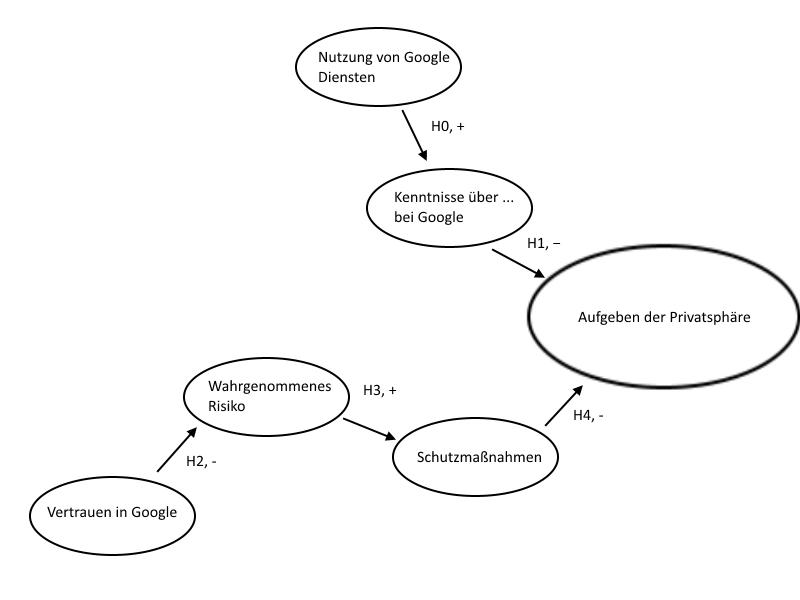
\includegraphics[scale=0.55]{images/bubbles}\\
\caption{Zusammenhang zwischen Kategorien und Hypothesen}\label{bubbles}
\end{figure}
	%%%%%%%%%%%%%%%%%%%%%%%%%%%%%%%%%%%%%%%%%%%%%%%%%%%%%%%%%%%%%%%%%%%%%%%%%%%%%%%
% 
% Prerequisites 
% Copyright (c) 2010 by tilo.mueller@rwth-aachen.de
% 
%%%%%%%%%%%%%%%%%%%%%%%%%%%%%%%%%%%%%%%%%%%%%%%%%%%%%%%%%%%%%%%%%%%%%%%%%%%%%%%

\chapter{Verwandte Arbeiten}
Die Problematik der Privatsphäre bei der Kommunikation mit Google Diensten ist ein Thema, zu dem es bereits einige Artikel und Forschungsarbeiten gibt. So beschreibt zum Beispiel \citet{tene2007google}, dass die größten Probleme der Privatsphäre sich in 6 Kategorien einteilen lassen.

Die erste Kategorie ist die Ansammlung der Daten. Das bedeutet, dass gesammelte und zu einem Gesamtbild zusammengefügte Daten viel mehr über einen Nutzer aussagen können, als er dies bei dem Veröffentlichen einer einzelnen Information erwartet. So wird als Beispiel angebracht, dass eine Suche nach \glqq French Mountains\grqq\ alleine nicht sehr aussagekräftig ist. Wenn aber kurz darauf noch nach \glqq ski vacation\grqq\ und \glqq gift to grandchild\grqq\ und weiterem gesucht wird, wird schnell klar, worum es sich bei der ersten Frage gehandelt hat. Wenn danach zum Beispiel noch nach \glqq disabled access\grqq\ gesucht wird, entwickelt sich ein sehr umfangreiches Bild über die Familie des Suchmaschinen-Nutzers. 

Der zweite Punkt ist die Verzerrung. Das heißt, dass Suchanfragen, wenn sie ohne Kontext gestellt sind, sehr schnell ein falsches Bild liefern können. Als Beispiel wird hier die Suchanfrage \glqq assassinate US president\grqq\ gezeigt - Behörden könnten hierbei schnell aufmerksam auf den Suchenden werden, obwohl sich jemand nur über die Geschichte von früheren Präsidenten informieren wollte.

Seine dritte Kategorie ist der Ausschluss. So dürfen sich Nutzer in Europa zwar ihre bei Google gespeicherten Informationen ausgeben lassen, da darüber aber nur wenige Menschen Bescheid wissen gilt Googles Datenbank letzten Endes als \glqq secret Database\grqq\ . 

Der vierte Punkt ist die \glqq sekundäre Nutzung\grqq . So wird durch die Verwendung von Google der Datenschutzrichtlinie zugestimmt, die es Google erlaubt, die Daten für weit mehr als der direkten Verwendung zu nutzen. Als Beispiel für eine sekundäre Nutzung kann die Werbung gesehen werden. 

Die letzten 2 Kategorien sind der Vertrauensbruch und die restlichen Probleme. In der Arbeit wird William Prosser zitiert, welcher sagt, dass der Nutzer in dem Veröffentlichen seiner privaten Daten eine Verletzung seines Vertrauens sieht. Unter den restlichen Problemen wird unter anderem die Überwachung genannt.

Als Analogie zu einer ähnlich tiefen Verbindung werden in \citet{debatin2009facebook} die Problematiken der Privatsphäre bei der Benutzung von Facebook untersucht. Genau wie Google ist Facebook ein Tool geworden, das alltäglich von vielen Nutzern verwendet wird und dabei sehr tief in die Privatsphäre eingreifen kann. Wie auch in dieser Arbeit geht es bei der Untersuchung zu einem großen Teil um die Verhaltensweisen der Nutzer und darum wie viel sie über die Konsequenzen ihres Verhaltensmusters wissen. So wird zum Beispiel gefragt, wie viele Nutzer der Meinung sind, sich mit den Einstellungen zur Privatsphäre in Facebook auszukennen. Außerdem werden sie gefragt, ob sie sich in der Lage fühlen, ihr Profil zumindest vor dem Zugriff Dritter zu schützen. Ähnliche Fragen werden auch in dieser Arbeit behandelt.

Eine weitere verwandte Arbeit ist \glqq Media coverage of online social network privacy issues in Germany: A thematic analysis\grqq\ von \citet{rizk2009media}. In diesem Paper wurde ein Teil der deutschen Medien auf das Thema \glqq Privatsphäre in sozialen Netzwerken\grqq\ durchsucht und die gesammelten Artikel wurden ausgewertet. Eines der Ergebnisse dieser Arbeit ist, dass es eine Beziehung zwischen Artikeln in den Medien und Änderungen in den Nutzungsbedingungen im Bereich Privatsphäre gibt. Das Paper kommt zu dem Schluss, dass diese Änderungen immer gleichzeitig mit, oder kurz nach großen Mengen an Artikeln zu dem Thema kommen.

Ein Begriff, der in den Ergebnissen dieser Arbeit immer wieder aufgetaucht ist, ist \glqq Personalisierte Werbung\grqq . Dieser Begriff wird auch in dieser Arbeit behandelt.

Auch \citet{Preibusch2007Ubiquitous} behandelt das Problem Privatsphäre in Sozialen Netzwerken. Der Artikel behandelt das Thema nicht nur im Bezug auf einzelne Personen, sondern auch im Bezug auf Privatsphäre im Netzwerk. Insbesondere geht es hier darum, dass Person A die persönlichen Daten von Person B missbrauchen kann, solange sie diese Person im Sozialen Netzwerk kennt. Diese Arbeit unterteilt dazu Vertraulichkeit in 4 Teile, Private Daten, Gruppen-Daten, Daten für das Netzwerk und öffentliche Daten. Sämtliche Daten ab \glqq Gruppendaten \grqq\ sind für Person A ersichtlich. Wenn diese Person nun bösartig ist, gibt es einen Konflikt mit der Privatsphäre. 

Um dieses Problem zu lösen, schlagen die Autoren eine Erweiterung des P3P (Platform for Privacy Preferences) vor. Mit dieser Erweiterung soll jeder Nutzer selbst festlegen können, auf welche Art sich Freundschaften zu anderen Nutzern auswirken. Zum Beispiel kann ein Nutzer private und öffentliche Freundschaften anlegen.

Eine weitere Arbeit mit ähnlichem Inhalt ist \citet{gross2005information}. Diese Arbeit listet einige Datenschutzauswirkungen auf, unter anderem werden \glqq Stalking\grqq , \glqq Re-Identifikation\grqq\ und der \glqq Fragile Datenschutz\grqq\ genannt.

Es existieren weitere Arbeiten mit ähnlichem Inhalt, wie zum Beispiel \citet{hintz2014AGB}, \citet{mahmood2011privacy} und \citet{hintzPhishing}, diese tangieren das Thema allerdings nur und werden hier deswegen nicht weiter ausgeführt.
	%%%%%%%%%%%%%%%%%%%%%%%%%%%%%%%%%%%%%%%%%%%%%%%%%%%%%%%%%%%%%%%%%%%%%%%%%%%%%%%
%
% methodology
% Copyright (c) 2010 by tilo.mueller@rwth-aachen.de
% 
%%%%%%%%%%%%%%%%%%%%%%%%%%%%%%%%%%%%%%%%%%%%%%%%%%%%%%%%%%%%%%%%%%%%%%%%%%%%%%%

\chapter{Methodik}

Die Studie wurde als Online-Umfrage entwickelt, mit dem Ziel, die Forschungsfragen zu beantworten. Dazu wurden die Forschungsfragen und die zugehörigen Hypothesen aufgestellt und mit diesen Mitteln der Fragebogen erstellt. 

Dieses Kapitel enthält die Einteilung der Konstrukte und der Hypothesen, die die Konstrukte in Verbindung bringen. 
Des weiteren wird die Fragebogenkonstruktion und die Rekrutierung der Teilnehmer beschrieben.

\section{Konstrukte}
\label{sec:categories}
Um die Forschungsfragen sinnvoll zu beantworten, wurden Konstrukte definiert, die Teilbereiche der Forschungsfrage abdecken sollen. Dabei wurde darauf geachtet, dass die Konstrukte gut auf die Forschungsfragen hinführen und durch Hypothesen aufeinander aufbauen können.

\begin{enumerate}
\item \label{itm:Kat0}\textbf{Nutzung von Google Diensten}: Das Nutzungsverhalten der Google Dienste von Seiten der Nutzer. Dieser Teil fragt vor allem allgemeine Daten zum Nutzungsverhalten ab. Darunter fallen unter anderem die Information, welche Dienste genutzt werden und wie viele Accounts die Nutzer haben.
\item \label{itm:Kat1}\textbf{Kenntnisse über Googles Datenschutz}: Angeeignetes Wissen über den Umgang mit personenbezogenen Daten bei Google, vor allem im Bezug auf die genutzten Dienste.
\item \label{itm:Kat2}\textbf{Vertrauen in Google}: Der Glauben, dass Google Charakteristiken zeigt, die Google davon abhalten, Verhalten zu zeigen, das dem Nutzer schadet.(vgl. \citet{mcknight2002impact}).
\item \label{itm:Kat3}\textbf{Wahrgenommenes Risiko für die Privatsphäre}: Der Glauben an auftretende negative Konsequenzen im Zusammenhang mit dem Preisgeben der Daten (vgl. \citet{kim2008trust}).
\item \label{itm:Kat4}\textbf{Bewusstsein über das Aufgeben der Privatsphäre}: Das Bewusstsein über den Verlust der Privatsphäre bei der Verwendung von Google Diensten.
\item \label{itm:Kat5}\textbf{Schutzmaßnahmen}: Verhalten des Nutzers zum Schutze der eigenen Privatsphäre.
\end{enumerate}

\section{Hypothesen}
Nach der Entwicklung der Konstrukte wurden Hypothesen aufgestellt, um diese miteinander in Verbindung zu bringen und die Forschungsfragen zu beantworten.
\begin{description}
\item[\label{itm:H0}\textbf{H1}]Je aktiver eine Person Google nutzt, desto mehr Kenntnisse über Googles Datenschutz bekommt sie.
\item[\label{itm:H1}\textbf{H2}]Je mehr eine Person über Googles Datenschutz weiß, desto bewusster ist ihr das Aufgeben der Privatsphäre.
\item[\label{itm:H2}\textbf{H3}]Je höher das Vertrauen in Google ist, desto geringer wird das Risiko eingeschätzt.
\item[\label{itm:H3}\textbf{H4}]Je höher das Risiko eingeschätzt wird, desto mehr Schutzmaßnahmen werden unternommen.
\item[\label{itm:H4}\textbf{H5}]Je mehr Schutzmaßnahmen eine Person verwendet, desto bewusster ist ihr das Aufgeben der Privatsphäre.
\end{description}

Durch die Umfrage sollen diese Hypothesen belegt oder widerlegt werden und somit die Zusammenhänge dargestellt und letzten Endes die Forschungsfrage beantwortet werden.

Der Zusammenhang zwischen den Kategorien und den Hypothesen soll anhand Grafik \ref{bubbles} verdeutlicht werden.
\begin{figure}[H]
\centering
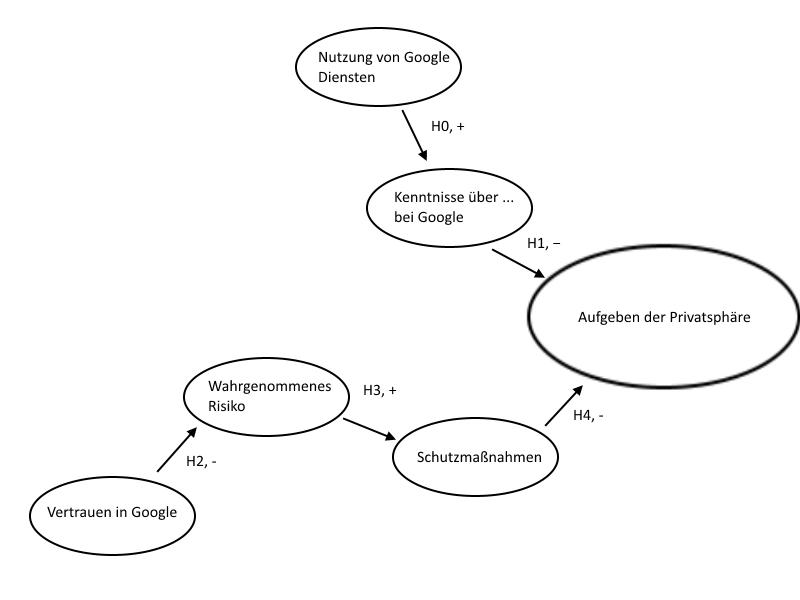
\includegraphics[scale=0.55]{images/bubbles}\\
\caption{Zusammenhang zwischen Kategorien und Hypothesen}\label{bubbles}
\end{figure}

\section{Fragebogenkonstruktion}
Zur Konstruktion des Fragebogens wurden die oben genannten Konstrukte und Hypothesen verwendet, um Fragen zu entwickeln. Diese Fragen sollten die Hypothesen möglichst gut beantworten und von Teilnehmern schnell und intuitiv lösbar sein. Das Ergebnis war eine Umfrage mit 39 Fragen. Diese Fragen wurden auf Seiten aufgeteilt, die ein schnelles und zielstrebiges Arbeiten durch den Fragebogens vereinfachen sollten.

Die Fragen sind zwar je einer der oben genannten Konstrukten zugeordnet, die Seiten in der Umfrage entsprechen aber nicht je einem Konstrukt. Dies hat den Zweck, dass Fragen die eventuell die Meinung der Teilnehmer beeinflussen könnten erst am Ende der Umfrage gestellt werden konnten.

Der letzte Teil der Umfrage ist eine Liste an demografischen Fragen, die eine Einordnung der Teilnehmer erleichtern soll. Am Ende dieses Teiles steht noch eine Frage nach Feedback zur Umfrage.
Bei der Umfrageerstellung wurde auf eine Bearbeitungsdauer von 10-15 Minuten kalkuliert. Bei den ersten Testteilnehmern wurde als tatsächliche Bearbeitungsdauer ein durchschnittlicher Wert von 12 Minuten gemessen, was dem erwünschten Wert entsprochen hat.

Abbildung \ref{catnumbers} zeigt auf, wie die Verteilung der Fragen auf die in Kapitel \ref{sec:categories} definierten Kategorien vorgenommen wurde und wie der Verlauf der Fragen in der Umfrage dargestellt wurde. Die Nummern der Fragen in der Grafik \ref{umldia} entsprechen den IDs der Fragen im Anhang (\ref{addendumquestions}). 

\begin{figure}[H]
\centering
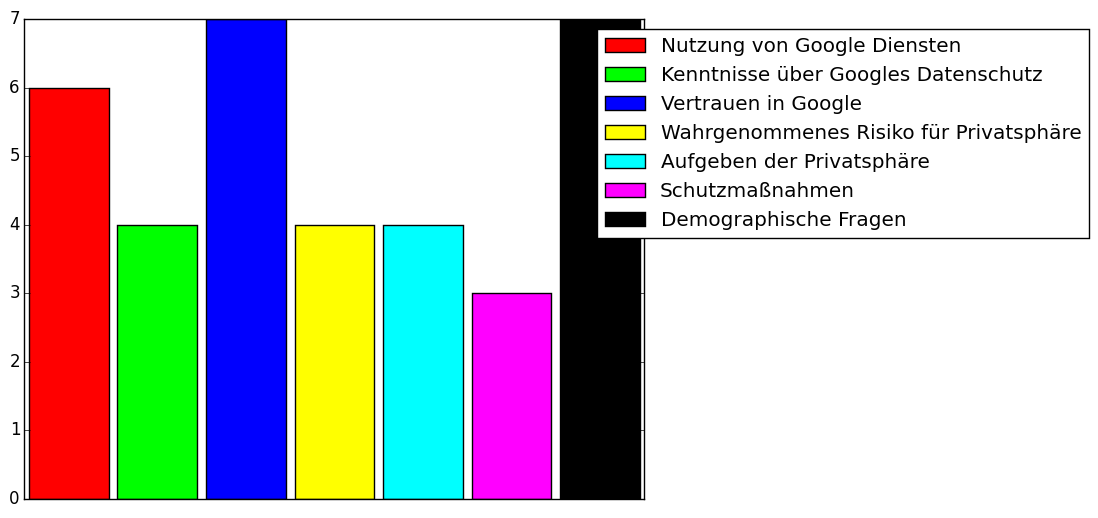
\includegraphics[width=\textwidth]{images/zahlenkategorien}\\
\caption{Anzahl der Fragen pro Kategorie in \ref{sec:categories}}\label{catnumbers}
\end{figure}

\begin{figure}[H]
\centering
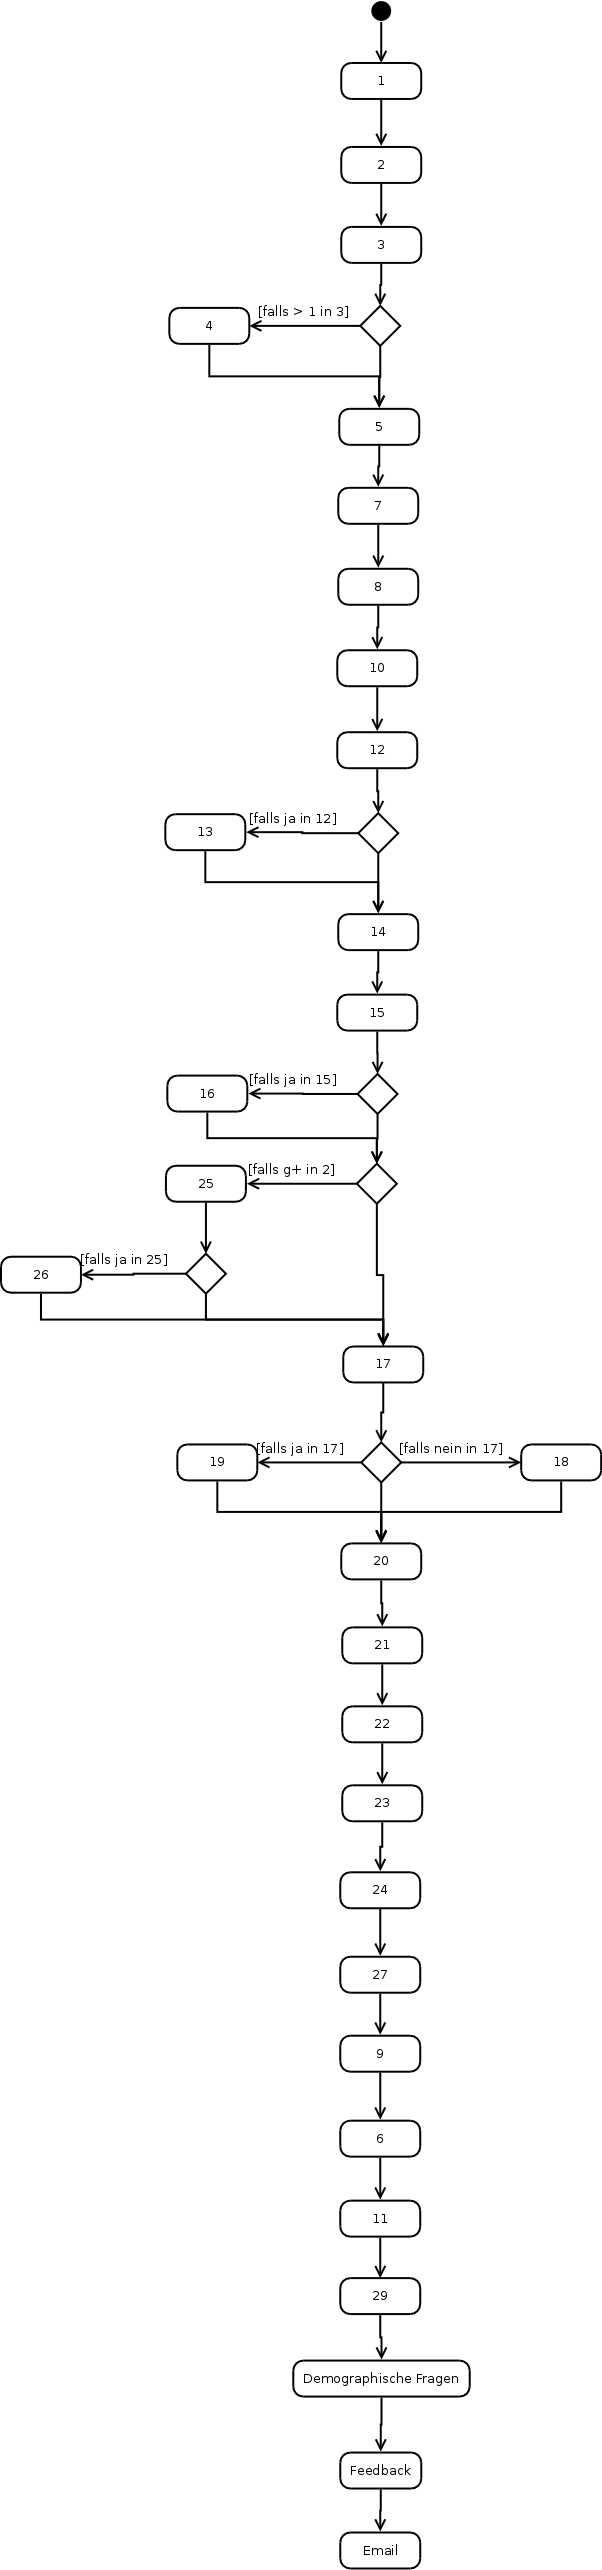
\includegraphics[height=\textheight]{images/umldia}\\
\caption{Anordnung der Fragen}\label{umldia}
\end{figure}


\section{Rekrutierung der Teilnehmer}
Die Umfrage wurde zuerst über Facebook und per Email über Familienmitglieder und Bekannte verteilt, mit der Angabe sie nach Möglichkeit auch weiter zu verteilen. Außerdem wurde die Umfrage in verschiedenen Foren verbreitet. Nachdem so schon eine relativ große Anzahl (knapp 200) an Antworten erhalten wurden, wurde die Umfrage noch über den E-Mail-Verteiler der Technischen Fakultät der Universität Erlangen-Nürnberg verbreitet.
	%%%%%%%%%%%%%%%%%%%%%%%%%%%%%%%%%%%%%%%%%%%%%%%%%%%%%%%%%%%%%%%%%%%%%%%%%%%%%%%
%
% results
% Copyright (c) 2010 by tilo.mueller@rwth-aachen.de
% 
%%%%%%%%%%%%%%%%%%%%%%%%%%%%%%%%%%%%%%%%%%%%%%%%%%%%%%%%%%%%%%%%%%%%%%%%%%%%%%%

\chapter{Ergebnisse}

Die Umfrage ergab 856 vollständig ausgefüllte Fragebögen. Dazu 164 nicht vollständig ausgefüllte, die laut dem Feedback Feld teilweise auf das Fehlen eines Zurück-Knopfes zurückzuführen sind, aber wohl eventuell auch einfache Abbrüche waren.

\section{Demographie}
Von den 856 Teilnehmern waren 204 (23,83%) weiblich, 613 (71,61%) männlich und 39 haben keine Angabe zu ihrem Geschlecht abgegeben. Die hohe Anzahl an männlichen teilnehmern liegt vermutlich daran, dass die Umfrage über den Email-Verteiler der Technischen Fakultät der Universität Erlangen-Nürnberg verteilt wurde, welche einen höheren Männer- als Frauenanteil hat.
Das durchschnittliche Alter beträgt 24.99 Jahre mit einer Standardabweichung von 9.23 Jahren. Das Maximum ist 99 Jahre und das Minimum 0 Jahre, wobei dies wohl beides Fehler sind - das Minimum könnte durch ein nicht ausgefülltes Feld entstanden sein, wohingegen die Person die das Maximum eingegeben hat mir persönlich gesagt hat dass dies ein Fehler war. Das untere Quartil ist 20, das Mittlere 23 und das Obere 26.
Interessant ist, dass trotz des niedrigen Wertes und der geringen Standardabweichung dennoch einige Fragebögen im Altersbereich von 45 bis 77 liegen. Diese müssen eventuell in der weiteren Auswertung gesondert betrachtet werden - denn selbst wenn ihre Anzahl nicht für statistisch exakte Aussagen reicht könnten hier dennoch interessante Ergebnisse gefunden werden.
Die nächste Frage fragte nach dem höchsten bisher erreichten Schulabschluss. Hier zeigt sich dass ein Großteil der Teilnehmer entweder gerade studiert oder bereits einen Abschluss im Studium erreicht hat. Abitur und Bachelor/Master/Diplom zusammen geben über 90% der Teilnehmer ab. Dagegen sind Hauptschulabschluss und Realschulabschluss zusammen nur knapp über 5.73%, was die Relevanz der Umfrageergebnisse ein wenig einschränkt, da sie nicht als allgemeingültig angesehen werden können sondern nur für einen speziellen Teil der Bevölkerung gelten. In einer zukünftigen Arbeit zu diesem Thema sollten eventuell speziell die Gruppen "Kein Abschluss", "Hauptschulabschluss" und "Realschulabschluss" betrachtet werden.
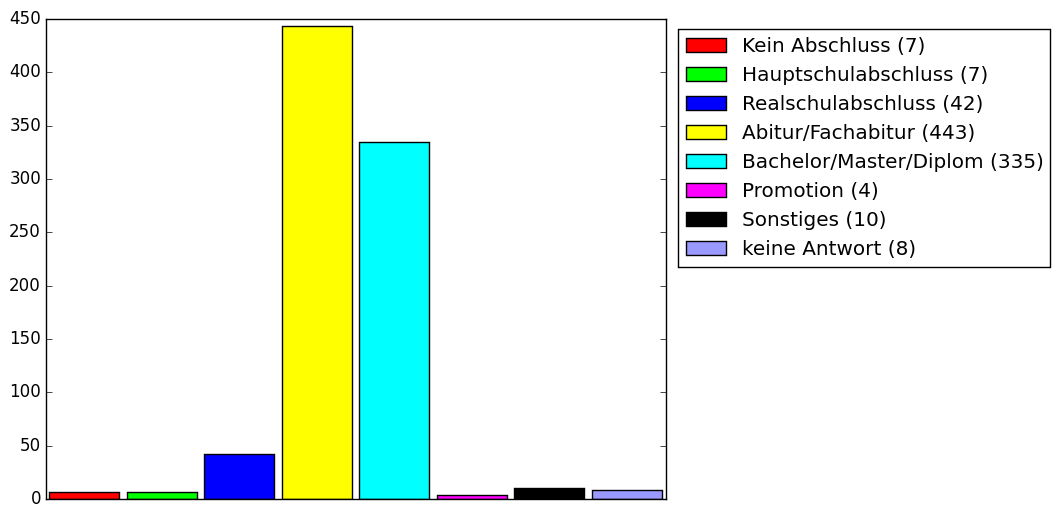
\includegraphics[scale=0.55]{images/schulabschluss}
Auch die folgende Frage zeigt das selbe Problem auf - 76.99% der Teilnehmer (659) waren zum Zeitpunkt des Ausfüllens Studenten. Dahingegen sind nur 1.99% in Ausbildung und 14.84% berufstätig.

\section{Hypothesen}

\section{Forschungsfragen}


\section{Sonstiges}

	%%%%%%%%%%%%%%%%%%%%%%%%%%%%%%%%%%%%%%%%%%%%%%%%%%%%%%%%%%%%%%%%%%%%%%%%%%%%%%%
%
% conclusion
% Copyright (c) 2010 by tilo.mueller@rwth-aachen.de
% 
%%%%%%%%%%%%%%%%%%%%%%%%%%%%%%%%%%%%%%%%%%%%%%%%%%%%%%%%%%%%%%%%%%%%%%%%%%%%%%%

\chapter{Fazit}

%Section		Depth
%\part			1
%\chapter		2
%\section 		3
%\subsection 		4
%\subsubsection 	5 	-> from here on it's not in default TOC anymore
%\paragraph	 	6
%\subparagraph 		7

\section{Zusammenfassung}
Aus den 856 ausgewerteten Fragebögen ergaben sich einige interessante Ergebnisse. Allerdings ist relevant, dass mit 71,6\% die Teilnehmerzahl überwiegend männlich war und über 90\% der Teilnehmer Studenten oder Personen mit Abitur waren. Diese beiden Fakten sorgen dafür, dass die Umfrage nicht repräsentativ für die Allgemeinheit ist.

Es lässt sich sagen, dass Google von den Nutzern sehr aktiv genutzt wird. Fast 90\% der Teilnehmer haben angegeben dass sie Google oft bzw. sehr oft nutzen.

Des weiteren kann man sagen, dass das Wissen der Nutzer über Google im in großen Teilen gut ist. Ein Großteil der Nutzer weiß zum Beispiel, dass Google personalisierte Suchergebnisse anbietet. Es gibt aber Lücken im Wissen, nur ein knappes Drittel der Teilnehmer weiß, dass man seinen Google Account löschen kann.

Das Vertrauen in Google ist eher gering - ein Drittel der Umfrageteilnehmer meint, dass ihre Daten bei Google nicht sicher sind.

Die Nutzer nehmen ein Risiko für ihre Privatsphäre wahr, so fühlen sich 85,9\% der Teilnehmer gegenüber Google nicht anonym.

In großen Teilen sind sich Nutzer über das Aufgeben ihrer Privatsphäre bewusst - viele Teilnehmer glauben zu wissen, dass Google viele ihrer privaten Daten, wie zum Beispiel Telefonnummer oder Wohnort kennt.

Tabelle \ref{hypothesenangenommen} zeigt, welche Hypothesen mit statistischer Signifikanz angenommen werden konnten und welche nicht belegt werden konnten.

Zu den Forschungsfragen lässt sich sagen, dass Nutzer wissen, dass Google ihre Daten sammelt, sie aber nichts oder nur wenig dagegen unternehmen. Hier zeigt sich wieder das typische Privatsphäre Paradoxon auf, welches im Bezug auf den Datenschutz ein bekanntes Problem ist.

\begin{table}
	\begin{tabular}[]{l | c }
	Hypothese & Angenommen\\\hline\hline
	Je aktiver eine Person Google nutzt,\\ desto mehr Kenntnisse über Googles Datenschutz bekommt sie. & Nein\\ \hline
	Je mehr eine Person über Googles Datenschutz weiß,\\ desto bewusster ist ihr das Aufgeben der Privatsphäre. & Ja\\ \hline
	Je höher das Vertrauen in Google ist,\\ desto geringer wird das Risiko eingeschätzt.&Ja\\\hline
	Je höher das Risiko eingeschätzt wird,\\ desto mehr Schutzmaßnahmen werden unternommen.&Nein\\\hline
	Je mehr Schutzmaßnahmen eine Person verwendet,\\ desto bewusster ist ihr das Aufgeben der Privatsphäre.&Nein\\\hline
	\end{tabular}
	\caption{Welche Hypothesen wurden statisch signifikant angenommen}\label{hypothesenangenommen}
\end{table}

\section{Ausblick}
In dem in dieser Arbeit behandelten Thema gibt es noch weite Bereiche zum weiteren Forschen.

Wie schon bei der Behandlung der demographischen Auswertung (\ref{sec:demo}) genannt, waren ein Großteil der Teilnehmer dieser Umfrage Studenten oder Personen, die ein Abitur als Abschluss hatten. Die Bevölkerungsgruppe, die als höchsten Bildungsabschluss einen Realschul- oder einen Hauptschulabschluss haben wurden kaum erreicht. Eine weitere Forschungsarbeit könnte in die Richtung gehen, dies weiter zu erforschen und sich z.B. im Besonderen auf diese Gruppen zu spezialisieren.

Des weiteren wäre es sinnvoll, Studien durchzuführen, bei denen das Wissen und die Taten der Nutzer direkt getestet werden. So wäre es zum Beispiel praktisch, Freiwillige zu fragen, ob man Einblick in die Sicherheitseinstellungen ihres Smartphones erhalten darf, um diese zu untersuchen. Alternativ könnte man Versuchsteilnehmer bitten, unter Aufsicht Sicherheitseinstellungen auf Google Seiten vorzunehmen.

Somit könnte direkt geprüft werden, wie viel die Teilnehmer tatsächlich eingestellt haben, oder ob ihre Aussagen dadurch beeinflusst sind, dass sie selbst gar nicht alle problematischen Bereiche kennen. Zum Beispiel sei hier angeführt, dass vielen Leuten eventuell gar nicht bewusst ist, dass allein dadurch, dass sie sich im selben WLAN befinden, oder einen ähnlichen GPS-Ort haben, bereits eine Verbindung zwischen ihnen und anderen aufgestellt werden kann. Fragen dieser Art wären eine weitere Untersuchung wert.

Weiterhin wäre es interessant zu erfahren, wie man das in Sektion \ref{sec:forschungsfragen} beschriebene Paradoxon der Privatsphäre lösen kann, beziehungsweise ob man es überhaupt lösen kann.


\chapter{Danksagung}
Mein Dank gilt Nadina Hintz und Zinaida Benenson, welche mich durch die Bachelorarbeit hindurch mit hilfreichen Vorschlägen begleitet haben.

Des weiteren danke ich natürlich meiner Familie, die mir während der Bachelorarbeit immer mit psychologischem Beistand beiseite gestanden sind und mir durch die stressige Zeit hindurch geholfen hat.

Zu guter Letzt danke ich den vielen Teilnehmern an der Umfrage dafür, dass sie Zeit aufgewandt haben um mir bei der Ausarbeitung dieser Arbeit zu helfen.
	%%%%%%%%%%%%%%%%%%%%%%%%%%%%%%%%%%%%%%%%%%%%%%%%%%%%%%%%%%%%%%%%%%%%%%%%%%%%%%%
%
% Anhang
% Copyright (c) 2010 by tilo.mueller@rwth-aachen.de
% 
%%%%%%%%%%%%%%%%%%%%%%%%%%%%%%%%%%%%%%%%%%%%%%%%%%%%%%%%%%%%%%%%%%%%%%%%%%%%%%%

\chapter{Anhang}

First chapter

%Section		Depth
%\part			1
%\chapter		2
%\section 		3
%\subsection 		4
%\subsubsection 	5 	-> from here on it's not in default TOC anymore
%\paragraph	 	6
%\subparagraph 		7


	\bibliography{citations}
	\bibliographystyle{plainnat}

\end{document}
